%%%%%%%%%%%%%%%%%%%%%%%%%%%%%%%%%%%%%%%%%%%%%%%%%%%%%%%%%%%%%%%%%%%%%%%%%%%%%%%
% intro.tex: Introduction to the thesis
%%%%%%%%%%%%%%%%%%%%%%%%%%%%%%%%%%%%%%%%%%%%%%%%%%%%%%%%%%%%%%%%%%%%%%%%%%%%%%%%
\chapter{Introduction}
\label{intro_chapter}
%%%%%%%%%%%%%%%%%%%%%%%%%%%%%%%%%%%%%%%%%%%%%%%%%%%%%%%%%%%%%%%%%%%%%%%%%%%%%%%%

%trite and boring. Cosmology has told us much about the universe. 



%%%%%%%%%%%%%%%%%%%%%%%%%%%%%%%%%%%%%%%%%%%%%%%%%%%%%%%%%%%%%%%%%%%%%%%%%%%%%%%%
% CMB Science {{{
%%%%%%%%%%%%%%%%%%%%%%%%%%%%%%%%%%%%%%%%%%%%%%%%%%%%%%%%%%%%%%%%%%%%%%%%%%%%%%%%
\section{Cosmic Microwave Background Polarization}
\label{sec:cmb_science}
%%%%%%%%%%%%%%%%%%%%%%%%%%%%%%%%%%%%%%%%%%%%%%%%%%%%%%%%%%%%%%%%%%%%%%%%%%%%%%%%

%In short: There was a big bang. Some gravity waves were probably generated. They may have left a signature polarization pattern on the \ac{CMB}. 

%The \ac{CMB} radiation is the oldest light in the universe, set free when the universe had cooled enough to allow protons and electrons to combine. 
%These \ac{CMB} photons, at a temperature of only 2.72~K, are a uniform background of radiation in all directions across our sky. 
%Measurements of the E-mode polarization (due to things that are not primordial gravity waves) have informed us about the evolution of universe. 
%Measurements of B-mode polarization due to primordial gravity waves would tell us about the earliest moments in the history of the universe. (and interesting things like the energy scale of inflation and may confirm or rule out expansion models).
%Measurements of B-mode polarization due to other stuff tells us about that other stuff. 
We seek to answer a fundamental question in cosmology:  how did the universe we know today (the galaxies, the stars, and the planets) come about?  
Merely $10^{-34}$ seconds after the big bang, the universe underwent a period of exponentially accelerated expansion, an epoch called inflation \cite{Guth1981} \cite{Linde1982} \cite{peebles} \cite{Spergel2007} \cite{Tegmark2006} \cite{PlanckXIII} \cite{PlanckXX}.  
380,000 years later, the universe became transparent to light when the baryon-photon plasma cooled enough for neutral hydrogen to form. 
Those photons, the oldest light in the universe, are called the \ac{CMB}.
The scalar primordial energy density perturbations imprinted a curl-free, or 'E-mode', polarization pattern on the \ac{CMB}. 
The E-mode polarization is at a level of 1~$\mu K$ and has been measured by several groups \cite{leitch2005} \cite{montroy2006} \cite{wu2007} \cite{sievers2007} \cite{nolta2009}. 

Inflation predicts the existence of a tensor stochastic background of gravitational waves which also left a curl component, or 'B-mode', in the polarization of the \ac{CMB}.  
The energy scale of inflation is proportional to the amplitude of this tensor B-mode polarization and it depends on the mechanism which drove the rapid acceleration \cite{Grishchuk1975} \cite{starobinsky1982} \cite{Rubakov1982} \cite{starobinskii1983} \cite{Abbott1984}.
Detection of the tensor B-mode polarization (or placing a constraint of 0.001 on the tensor to scalar ratio, r) is important because it would confirm (or rule out) the single field slow-roll inflation model \cite{Abazajian2015}.
Across the sky, the polarized thermal emission from galactic dust is the largest foreground above 100~GHz \cite{PlanckXXX} and will need to be subtracted in order to extract the tensor B-mode signal from the \ac{CMB}. 
%Measuring r at this level will require incredible sensitivity. 
%And it will require subtracting pesky foregrounds like polarized galactic dust. 
There is also a B-mode polarization pattern in the \ac{CMB}, at smaller angular scale, due to gravitational lensing of the E-mode polarization \cite{polarbear2014} \cite{naess2014} \cite{keisler2015}.
Figure~\ref{fig:cmb_spectra} shows the predicted E- and B-mode polarization power spectra of the \ac{CMB} for the \textcolor{red}{XXX model} assuming r=0.05.


%The tensor to scalar ratio, r, quantifies the strength of gravity waves during inflation.  
%In the lambda cold dark matter model,
%The energy scale of inflation, $V^{1/4}$, is proportional to the amplitude of B-mode polarization
%\begin{equation}
%V^{1/4} = 3.7 \times 10^{16}   r^{1/4}   GeV
%\end{equation}
%where $V$ is the inflaton potential and r is the tensor to scalar ratio. 
%
%\textcolor{red}{assuming a lamba-cdm cosmology 
%what is r? r = 0.05 (should I talk more about what this means?? what cosmological models are ruled out? which are favored and why are they favored (because they're simple)?)
%what is tau?
%also. ends too abruptly. continue motivating.
%e.g. you must mention the polarized galactic dust foregrounds which contaminate signal
%}

%Such a limit would have significant consequences because it rules out the simplest, most favorable models of inflation.  
%The theory of inflation posits the universe underwent exponential expansion in only 
%predicts gravity wave were generated at the time of inflation. 
%B-mode polarization pattern of the \ac{CMB} is a direct probe of the physics of inflation. 


\begin{figure}[htbp]
\begin{center}
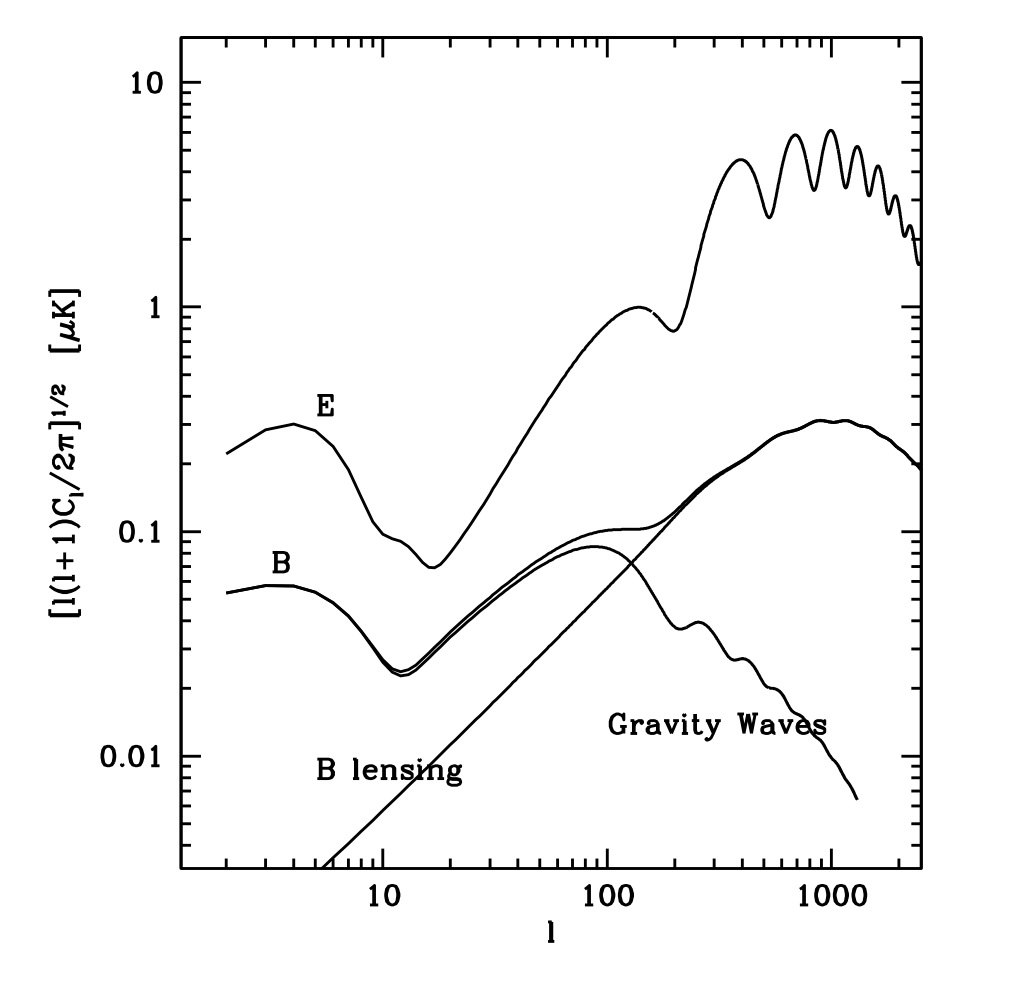
\includegraphics[height=3.2in]{figures/predicted_power_spectra.png}
\caption[CMB power spectra]{The theoretical prediction of the E- and B-mode power spectra of the \ac{CMB}. The E-mode polarization has been measured to high accuracy. The B-mode power spectra is expected to have a component due to lensing, which has been measured, and a component due to primordial gravity waves, which hasn't yet been detected with high confidence. This plot shows the level of the B-mode polarization assuming a tensor-to-scalar ratio of r=0.05, which is near the current upper limit set by Planck and Keck Array. 
\label{fig:cmb_spectra} }
\end{center}
\end{figure}



%%%%%%%%%%%%%%%%%%%%%%%%%%%%%%%%%%%%%%%%%%%%%%%%%%%%%%%%%%%%%%%%%%%%%%%%%%%%%}}}

%%%%%%%%%%%%%%%%%%%%%%%%%%%%%%%%%%%%%%%%%%%%%%%%%%%%%%%%%%%%%%%%%%%%%%%%%%%%%%%%
% High-Altitude Ballooning {{{
%%%%%%%%%%%%%%%%%%%%%%%%%%%%%%%%%%%%%%%%%%%%%%%%%%%%%%%%%%%%%%%%%%%%%%%%%%%%%%%%
\section{High-Altitude Ballooning}
\label{sec:balloons}
%%%%%%%%%%%%%%%%%%%%%%%%%%%%%%%%%%%%%%%%%%%%%%%%%%%%%%%%%%%%%%%%%%%%%%%%%%%%%%%%

%Explain the motivation for flying a CMB telescope from a high-altitude balloon. 
%The advantages. 
%The disadvantages. 

High-altitude balloons, relative to satellites, are powerful platforms for achieving low budget and fast astrophysical studies. 
The high altitude observation environment also enables measurement of frequencies inaccessible on the ground. 
%why shouldn't I say which frequencies these are?
The high frequency data are critical to determine the spectra of dust so the dust foreground can be subtracted from the signal. 

One challenge in ballooning is the length of observation. 
Figure~\ref{fig:flight_trajectory} shows the \ac{EBEX} flight path. 
The average \ac{LDB} flight duration from McMurdo, Antarctica is 18~days, and the longest flights have lasted more than 40~days.  
While this is much shorter than the operation time of a ground-based telescope, the factor of \textcolor{red}{$\sim$XXX} increase in instantaneous detector sensitivity in the space-like environment can make a high-altitude balloon experiment worthwhile. 
%can you be quantitative? can you just approximate? if apexsz-150 load was 15pW (target 30pW) and ebex load was 2.5pW(target 7.5pW) and sensitivity is dominated by photon nep and photon nep is proportional to square root of Popt ... then nep_apex/nep_ebex = sqrt(15/2.5) or sqrt(30/7.5)
Section~\ref{sec:detector_design} discusses the detector design modifications we performed to optimize the detector sensitivity for a space-like environment. 
The typical flight altitude is around 36~km, above approximately 98\% of the atmosphere. 
At this altitude, and at an elevation of 45$^\circ$, the radiative load from the atmosphere is less than 0.04~pW for the 150 and 250~GHz observation bands and around 2~pW for the 410~GHz observation band \cite{Bao2015}. 
%sure would be nice if you could say what it is on the ground and say what is assumed about precipital water vapor

%Shaul says this doesn't go anywhere. he's right. I don't want to make it go anywhere for now. just remove...
%Another challenge in ballooning is the limited bandwidth available for transmitting data to and from the payload. 
%This makes sending compact commands to operate the entire detector array essential and  recovering the payload of critical importance. 

%There are several advantages to Antarctic balloon flights. 
Antarctic flights offer the longest flights on the planet with the highest probability of data recovery. 
Favorable wind patterns set up in the austral summer to bring the balloon around in a circle, usually staying over the continent, and coming back to roughly where it began, see Figure~\ref{fig:flight_trajectory}. 
The continent is sparsely populated so there is little danger of injuring anyone or anything. 
Also, during the austral summer in Antarctica, the payloads are exposed to the sun around the clock. 
The batteries need to provide just enough power to make it through launch and ascent and then the sun exposure allows for constant charging of the solar panels to power the experiment. 
This is important for minimizing the weight of the payload. 
%can you say why you want to minimize the weight of the payload?

\begin{figure}[htbp]
\begin{center}
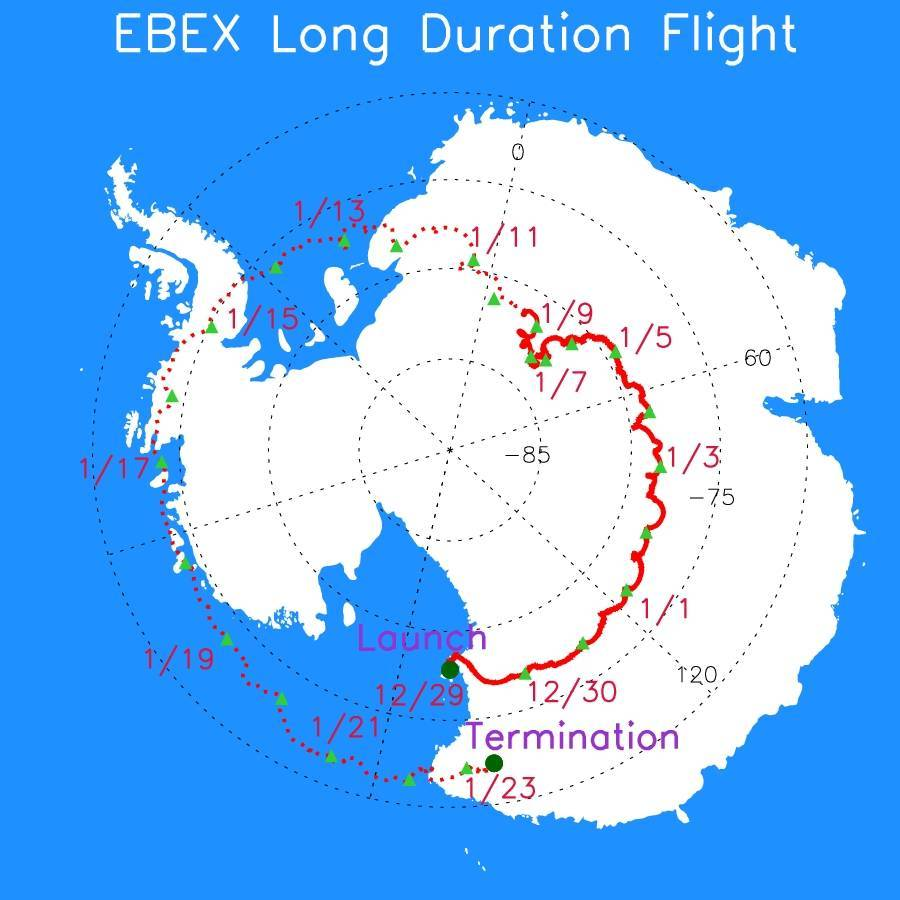
\includegraphics[width=0.6\columnwidth]{figures/ebex_trajectory.jpg}
\caption[EBEX flight trajectory]{The flight path \ac{EBEX} followed over Antarctica. On January 9, the trajectory line goes from solid to dashed because, exactly as predicted, the liquid helium ran out after twelve days and so \ac{EBEX} stopped collecting data. 
\label{fig:flight_trajectory} }
\end{center}
\end{figure}

%%%%%%%%%%%%%%%%%%%%%%%%%%%%%%%%%%%%%%%%%%%%%%%%%%%%%%%%%%%%%%%%%%%%%%%%%%%%%}}}



%%%%%%%%%%%%%%%%%%%%%%%%%%%%%%%%%%%%%%%%%%%%%%%%%%%%%%%%%%%%%%%%%%%%%%%%%%%%%%%%
% EBEX {{{
%%%%%%%%%%%%%%%%%%%%%%%%%%%%%%%%%%%%%%%%%%%%%%%%%%%%%%%%%%%%%%%%%%%%%%%%%%%%%%%%
\section{The E and B EXperiment}
\label{sec:ebex}
%%%%%%%%%%%%%%%%%%%%%%%%%%%%%%%%%%%%%%%%%%%%%%%%%%%%%%%%%%%%%%%%%%%%%%%%%%%%%%%%

\ac{EBEX} was a balloon-borne telescope flown on an Antarctic long duration balloon flight supported by \ac{NASA}'s \ac{CSBF}. 
\ac{EBEX} was designed to measure the polarization of the \ac{CMB}.
The goals of the project were to:
\begin{itemize}
\item measure or put an upper limit on the B-mode polarization signal due to primordial gravitational waves%, a tensor-to-scalar ratio 
\item measure the polarization of the galactic foregrounds, in particular galactic dust
\item measure the B-mode polarization signal due to lensing and effectively separate it from the signal due to gravity waves
\item measure the E-mode polarization signal
\item provide a milestone in the implementation and testing of detectors, detector readout, optics, and polarimetry techniques being considered for a future NASA CMB polarization satellite
\end{itemize}
This thesis contributes to the final item, in particular, the implementation and testing of the detectors and their readout. 

\ac{EBEX} had three observation frequency bands, designed to be centered around 150, 250, and 410~GHz. 
%There were the highest number of channels in the \ac{CMB} peak channels, the low frequency band.
The lowest frequency band was the \ac{CMB} observation band. 
The higher frequency bands were included to measure the polarization of the galactic dust so it could be accurately subtracted from the \ac{CMB} observation band. 
Foreground subtraction was predicted to be necessary because, even in the planned observation clean sky patch of $\sim$400 deg$^2$, the dust was predicted to dominate the primordial gravitational B-mode signal \cite{Bao2015}. 
%Don't talk about this here? Don't talk about it at all?
%The motor controller overheated during flight, so the scan pattern was actually determined by the rotation of the gondola hanging from the balloon. 
%The final observation patch was a $\sim$6000 deg$^2$ strip of constant declination.%between -66$^\circ$ and -40$^\circ$

\ac{EBEX} was an off-axis Gregorian
%dragone ???
 telescope.
The outer frame carried the pointing control, the experiment power, and the flight control computer. 
The inner frame carried the 1.5~m primary mirror, the 1~m secondary mirror, the cryostat, and the readout electronics. 
The left panel of Figure~\ref{fig:outer_frame} is a model of \ac{EBEX} and the right panel is the instrument in a similar configuration to the model, but is a photograph of it hanging on the launch pad \cite{EBEXPaper3}. 
The majority of the telescope was surrounded by mylar-covered baffling protecting it from the light of the sun. 
The solar panels were mounted to the back of the telescope to be constantly charging while the telescope front was set to point anti-sun. 

\begin{figure}[htbp]
\begin{center}
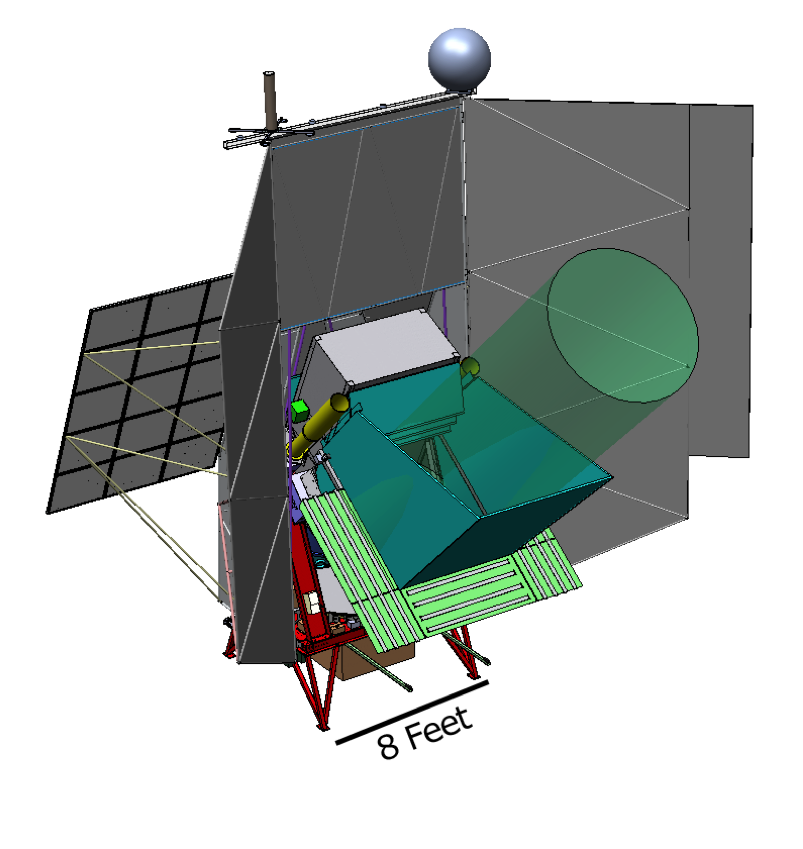
\includegraphics[height=3.2in]{figures/ebex_model.png}
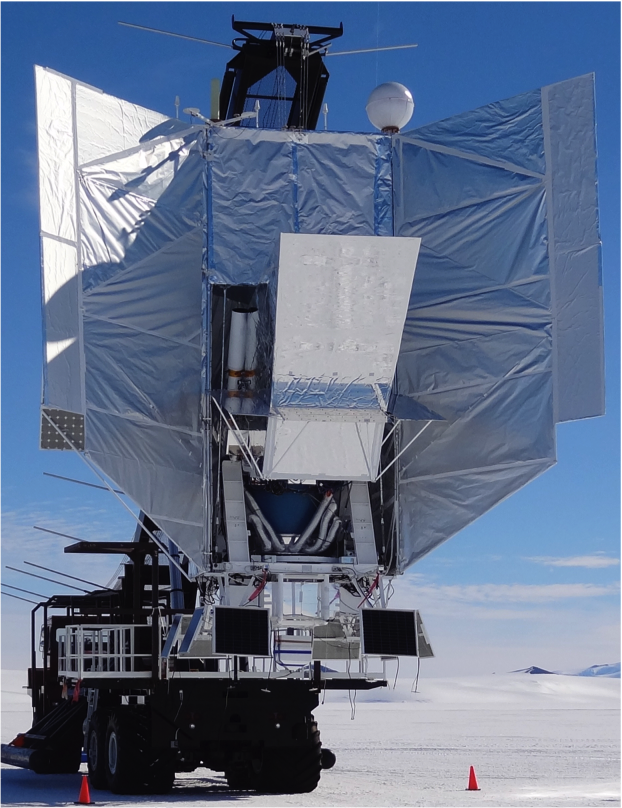
\includegraphics[height=3.2in]{figures/ebex_hanging.png}
\caption[EBEX model and photograph]{Left: Model of \ac{EBEX} \cite{Zilic2014}. There is a green cylinder showing the path of light entering the telescope via the teal scoop. Neon green radiation panels, to dissipate power from the readout electronics at float, surround the scoop. The solid grey panels are the mylar-covered baffling. Attached to the rear, a single solar panel is visible as a black grid on a grey rectangle. Right: Photograph of \ac{EBEX} hanging on the launch vehicle in Antarctica. Photograph courtesy of Asad Aboobaker. 
\label{fig:outer_frame} }
\end{center}
\end{figure}

The path of light through the telescope is shown in Figure~\ref{fig:optical_path}. 
Light bounced off the primary mirror and was reflected into the cryostat by the secondary mirror. 
The light entered the cryostat via an \ac{UHMWPE} 1.0~mm window, transparent to mm-wave light. 
On the ground, this window under vacuum would have deflected enough to damage the filters beneath it. 
To prevent that from happening, the telescope had a double window mechanism mounted to the top of the cryostat, Figure~\ref{fig:double_window} \cite{Zilic2017}. 
On the ground, there was an additional \ac{UHMWPE} window of thickness 12.7~mm under vacuum above the thin window. 
At float, the thick window was rolled back. 
Once the light entered the cryostat, it was filtered and passed through a half-wave plate continuously rotating at 1.2~Hz. %1.235~Hz
There was a polarizing grid through which half of the light passed and was focused onto the horizontal focal plane.
The other half of the light reflected off of the polarizing grid and was focused onto the vertical focal plane. 
Figure~\ref{fig:cryo_innards} shows a model of the interior of the cryostat and a photograph of the optical elements housed inside the optics box \cite{EBEXPaper1}. 

\begin{figure}[htbp]
\begin{center}
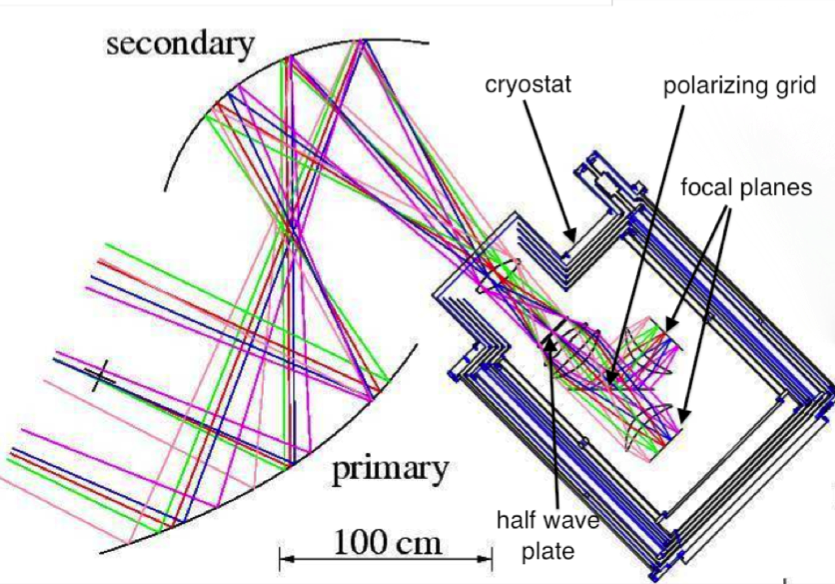
\includegraphics[height=3.2in]{figures/ebex_optical_path.png}
\caption[EBEX optical path]{Path of light, the multicolored bundle of rays, through \ac{EBEX}. It first strikes the primary mirror, is reflected onto the secondary mirror, passes through the cryostat window, and is focused onto the cold aperture stop where the half-wave plate is mounted. From there it is imaged onto the two focal planes. 
\label{fig:optical_path} }
\end{center}
\end{figure}

\begin{figure}[htbp]
\begin{center}
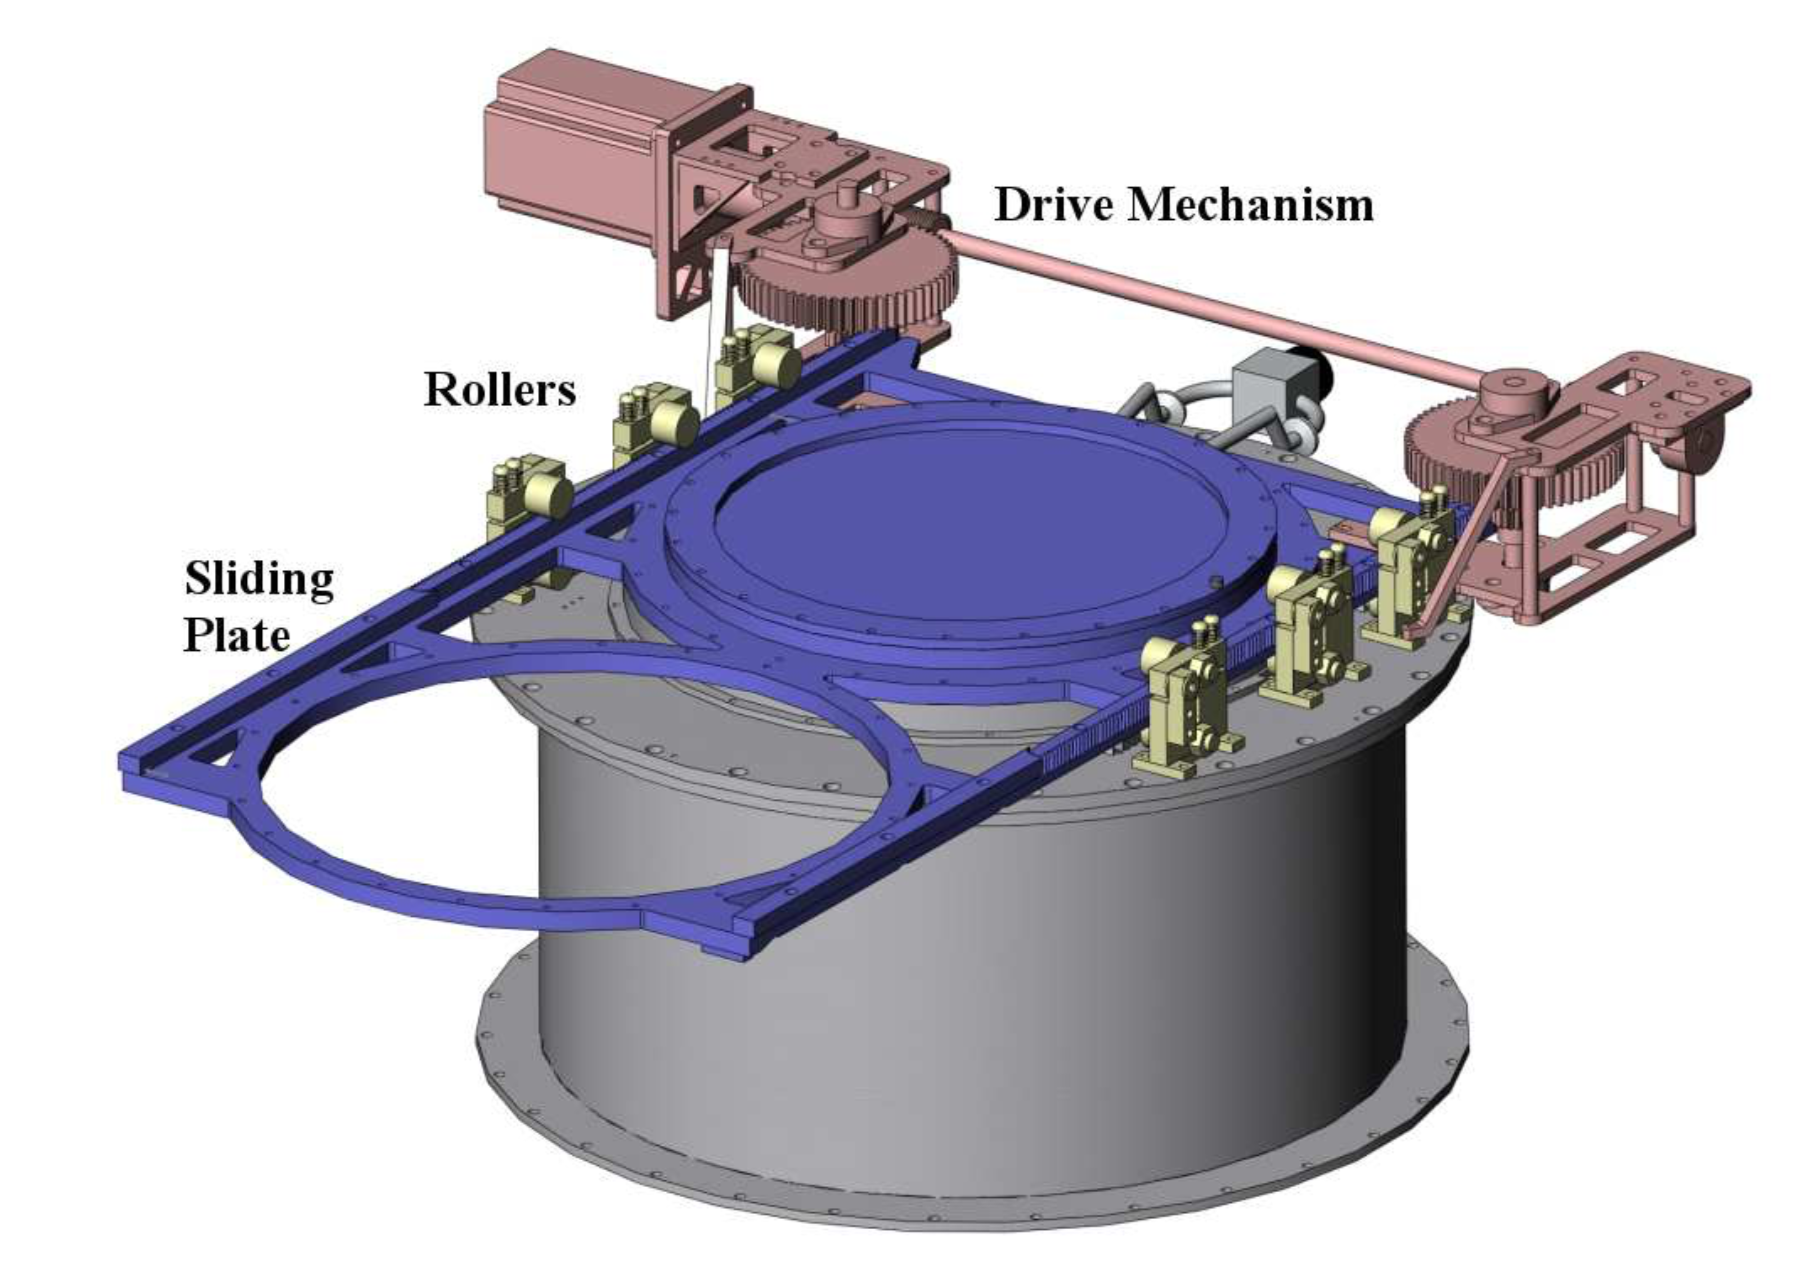
\includegraphics[height=3.2in]{figures/double_window.png}
\caption[EBEX double window]{The \ac{EBEX} double window design. On the ground, there were two windows under vacuum. At float, the thick 12.7~mm window was rolled back and only the thin 1.0~mm window remained in the light path. \cite{Zilic2014}
\label{fig:double_window} }
\end{center}
\end{figure}

\begin{figure}[htbp]
\begin{center}
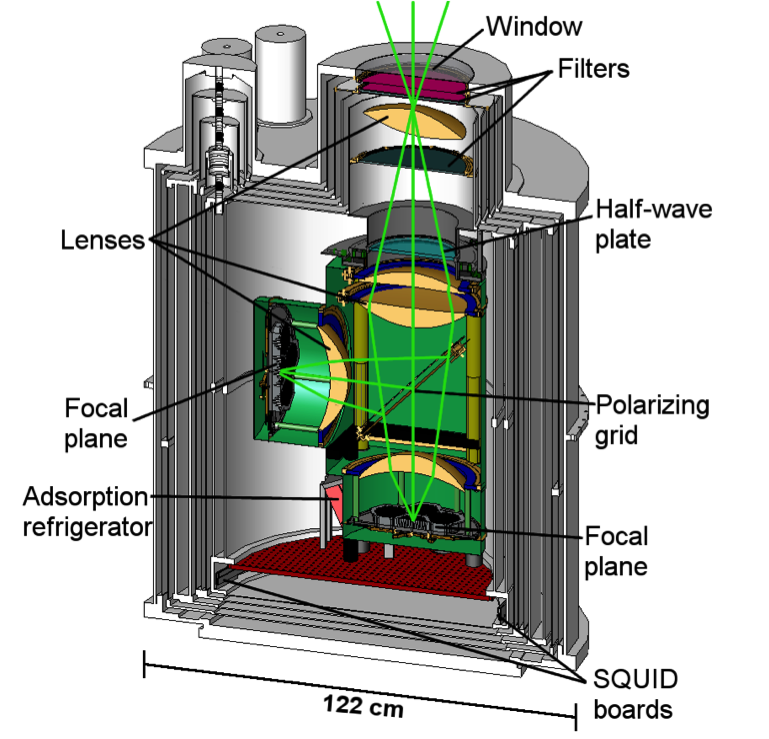
\includegraphics[width=0.48\columnwidth]{figures/ebex_cryostat_cross_section.png}
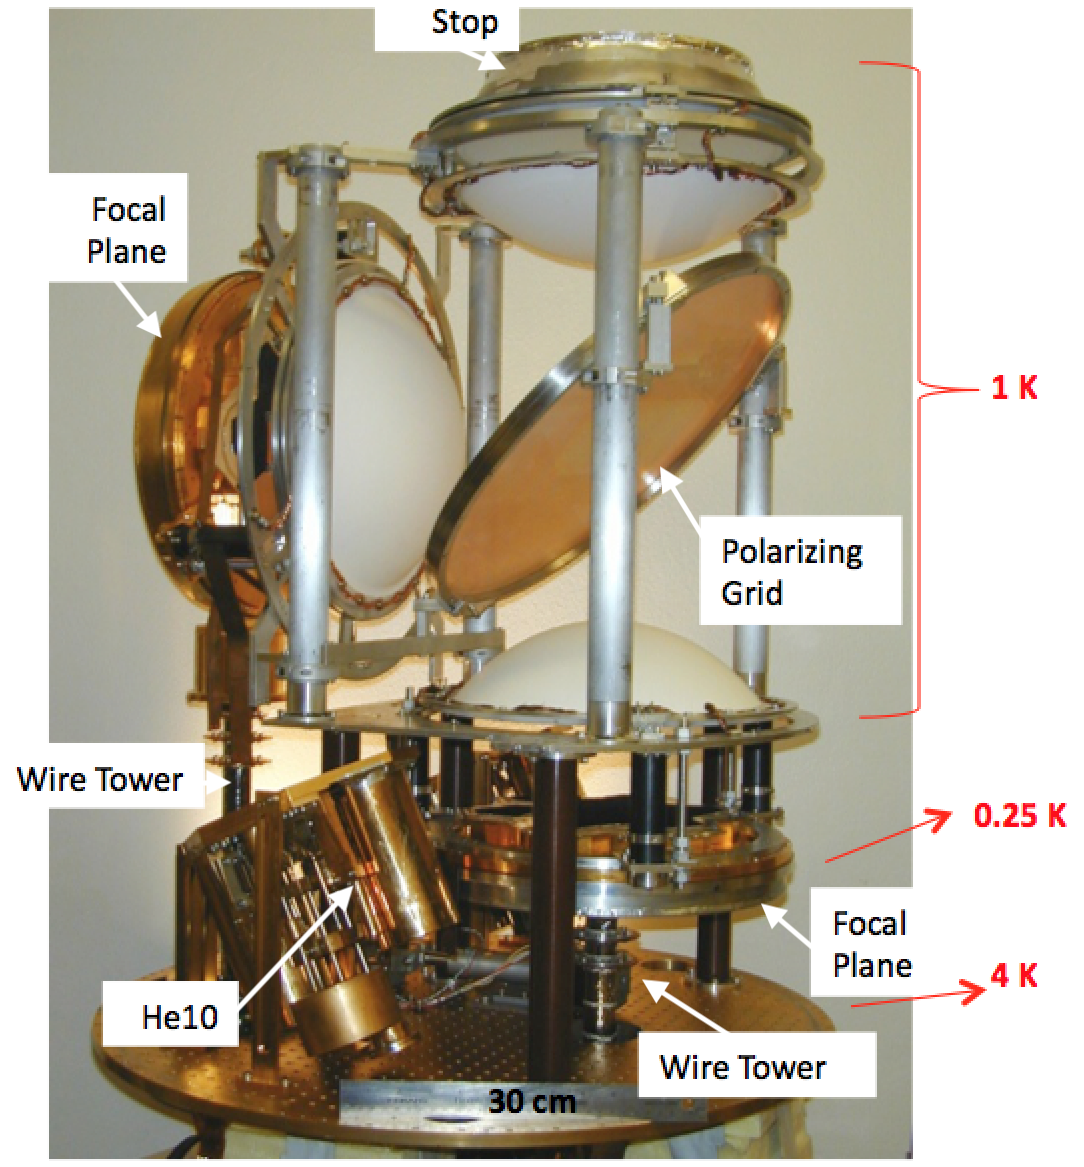
\includegraphics[width=0.48\columnwidth]{figures/cryo_innards.png}
\caption[EBEX cryostat cross section and interior optics elements]{Left: Cross-section of \ac{EBEX} cryostat model. The grey shells are the toroidal cryogen tanks and vapor cooled shells. Light is represented as neon green rays. The light passes through the window, the filter stack, the continuously rotating half-wave plate, lenses, and is split at the polarizing grid. Half of the photons continue to the horizontally mounted focal plane below and the other half are reflected to the vertically mounted focal plane to the side. Right: Photograph of \ac{EBEX} cold plate and optics elements beneath the half-wave plate. The half-wave plate sits above the stop at the top of the stack shown. The orange circle at a 45$^\circ$ angle is the polarizing grid. The focal planes are the gold plated enclosures with the wiring towers beneath them. The structures are supported by thin walled vespel legs. One of the Simon Chase helium adsorption refrigerators is visible mounted to the cold plate on the lower left of the photograph. 
\label{fig:cryo_innards} }
\end{center}
\end{figure}

%PROVIDING TOO MANY DETAILS????

There were two focal planes and each focal plane consisted of seven silicon wafers of detectors, four at 150~GHz, two at 250~GHz, and one at 410~GHz, see Figure~\ref{fig:focal_plane} \cite{EBEXPaper2}.
Each wafer had 140~detectors fabricated via thin metal deposition and optical lithography. 
See section~\ref{sec:yield} for a discussion of the detector yield achieved.  
Each wafer was mounted to an invar plate with a thin layer of warmed Apiezon N grease. 
The invar plate was screwed to an aluminum wafer/LC board mount and an alignment jig was used to to position the wafer relative to dowel pin holes on the waveguide array. 
%The dowel pin holes aligned the wafer with the waveguide array. 
The invar plates were heat sunk to a Simon Chase helium adsorption fridge which cooled the wafers to $\sim$250~mK.  

\begin{figure}[htbp]
\begin{center}
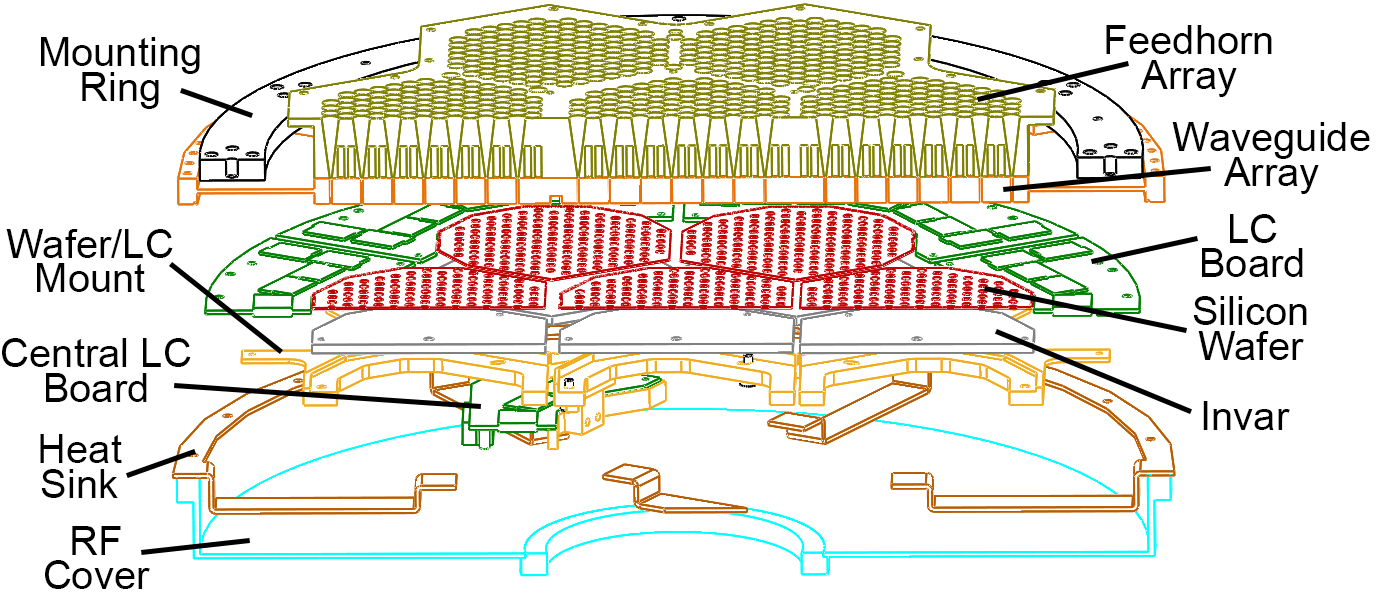
\includegraphics[height=2.0in]{figures/focal_plane_outline_central_labeled.png}
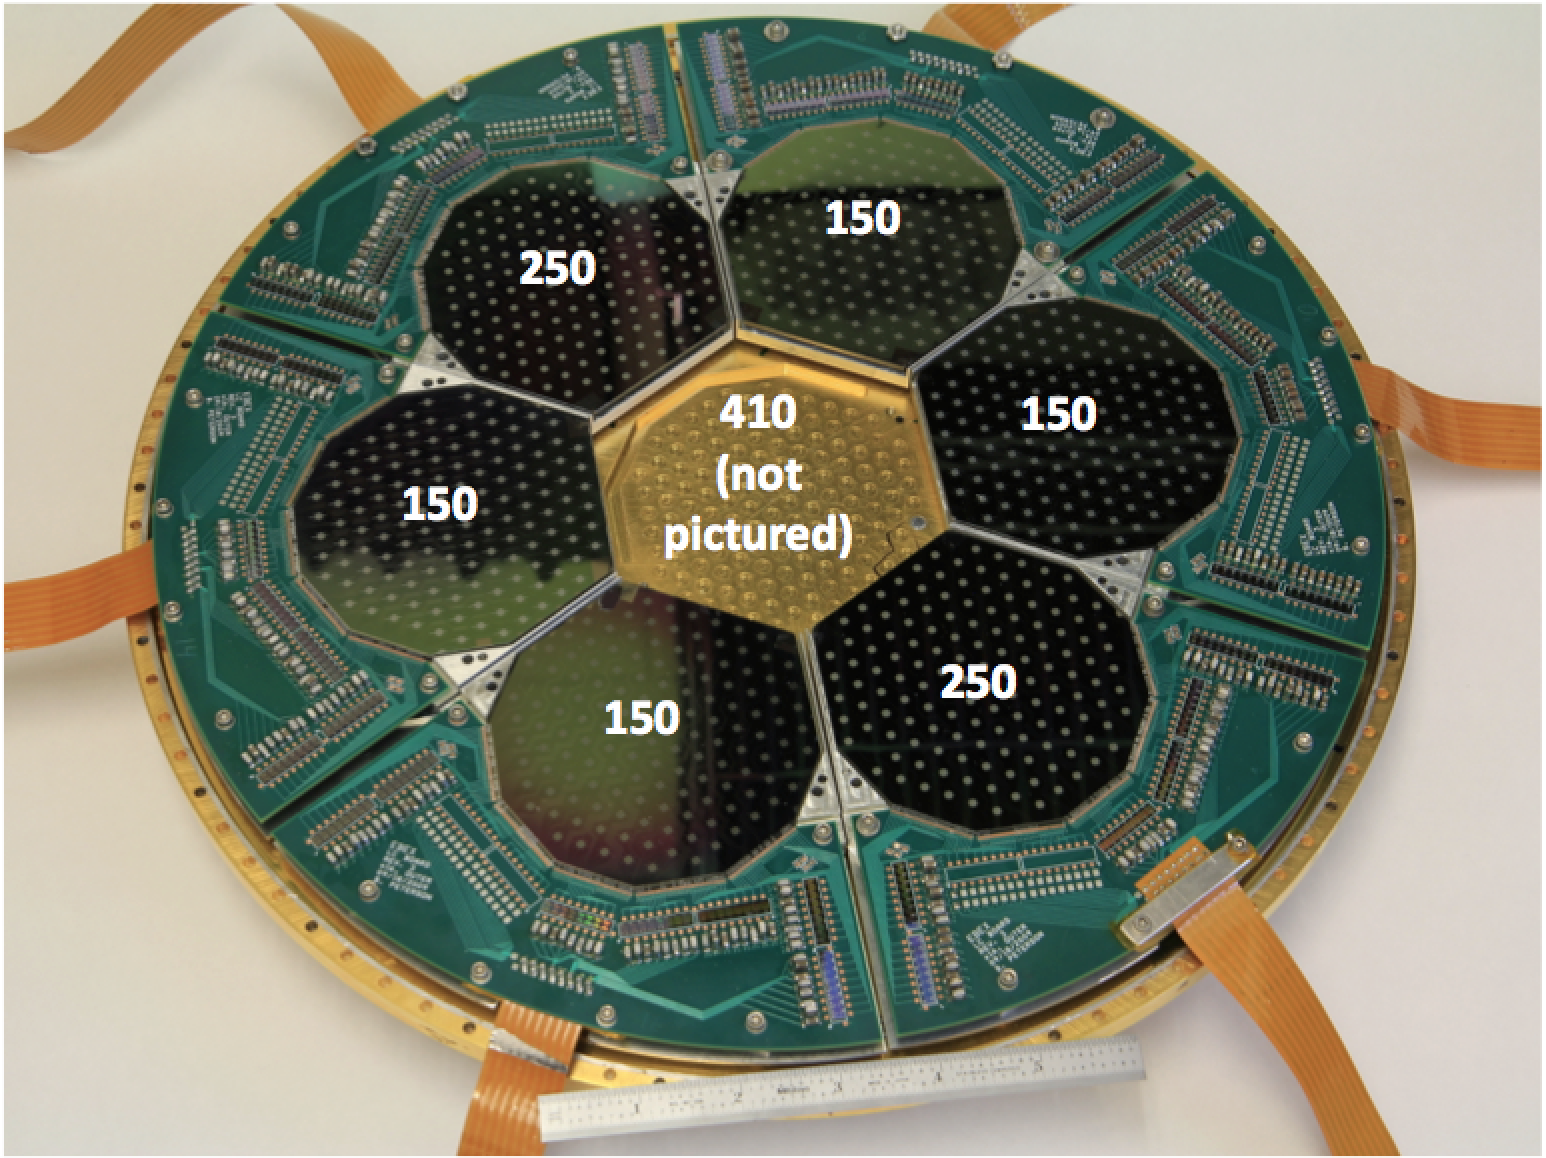
\includegraphics[height=2.0in]{figures/focal_plane_photo.png}
\caption[EBEX focal plane]{Top: An exploded model of the focal plane. Light passes through low pass filters (not pictured), to the feedhorns and waveguides, to the bolometers in their integrating cavities below. Each wafer is mounted to an invar plate which is attached to an aluminum wafer/\ac{LC} mount. The wafer is wirebonded to an \ac{LC} board. Note, the central \ac{LC} board is offset into the space behind the wafer/\ac{LC} mounts. There is a copper heat sink ring around the perimeter and attaching to each invar plate. The entire assembly is enclosed by an RF cover. Bottom: The silicon detector wafers wirebonded to their \ac{LC} boards. The wafer assemblies are sitting atop the gold-plated waveguide and horn array. The copper pigtails are leading off the edge of the photograph, but when fully assembled are routed through the wiring towers. The 410~GHz wafer with its offset \ac{LC} board is not included in the photograph. 
\label{fig:focal_plane} }
\end{center}
\end{figure}

The detector signals were read out using \ac{DfMUX} electronics, Figure~\ref{fig:dfmux}.
The detectors were nominally grouped into combs of sixteen detectors per pair of wires leading from the focal plane. 
Each detector was wired in series with a 24~uH inductor and ceramic capacitor between $\sim$0.9 and 30~nF on the \ac{LC} board. 
This gave a comb of sixteen resonant frequencies from 200 to 1200~kHz, with spacing of roughly 65~kHz. 
The signal from each comb was amplified by a NIST 100 series array \ac{SQUID}. 
The \ac{DfMUX} carriers, and a 0.03~$\Omega$ resistor, provided each detector's voltage bias at its resonant frequency and the \ac{DfMUX} nullers canceled the bias signal at the input of the \ac{SQUID}. 
To bring the comb of signals from the 250~mK \ac{LC} boards to the 4~K \ac{SQUID}s, there was a short pair of kapton encased flattened copper wires attached to a pair of low-inductance parallel kapton encased flattened niobium titanium wires.
A twisted pair of 150~mm long manganin wire exited the cryostat carrying the signal from the 4~K squids to the room temperature \ac{SQUID} controller board. 
The \ac{DfMUX} board demodulated the signal and the flight control computer recorded all of the data. 

\begin{figure}[htbp]
\begin{center}
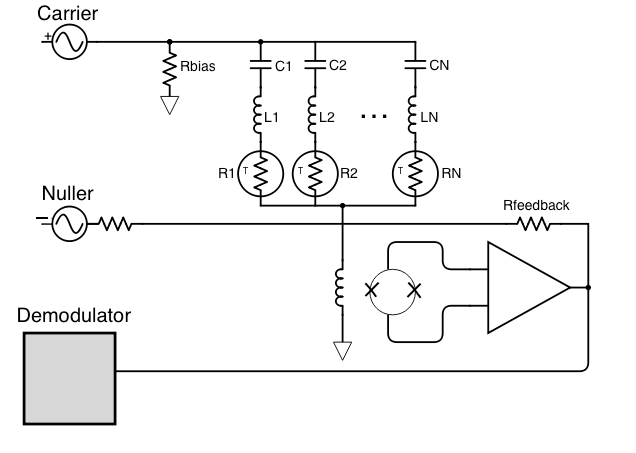
\includegraphics[width=0.6\columnwidth]{figures/dfmux_schematic.png}
\caption[DFMUX schematic]{Schematic of readout electronics. 
\label{fig:dfmux} }
\end{center}
\end{figure}

%Within each focal plane, \textcolor{red}{talk about 
%\begin{itemize}
%\item the wafer mounting procedure. 
%\item the readout procedure
%\item somewhere, don't you need to say how things get cold? and why?
%\end{itemize}
%}

%\textcolor{red}{in Section~\ref{sec:detector_characterization} you say "the wafer was mounted and coupled to the readout electronics as was done for flight, Section~\ref{sec:ebex}". 
%So. 
%Here. You need to describe the wafer mounting procedure and how the signal is read out. 
%Perhaps you will make a subsection and reference that subsection when referencing how the wafer was mounted and coupled to readout?}




% \textcolor{red}{Do you want to include the spectra we thought we could get observing the patch we thought we were going to observe?}
 
 %\textcolor{red}{Do you want to include the patch we thought we were going to observe? And the swath of sky we did observe?}

%The launching, tracking, and recovering were done by ...
%Describe cryostat, gondola. 





%\textcolor{red}{Do you want/need to include the 410 wafer mount stuff?}
 
%%%%%%%%%%%%%%%%%%%%%%%%%%%%%%%%%%%%%%%%%%%%%%%%%%%%%%%%%%%%%%%%%%%%%%%%%%%%%}}}





%%%%%%%%%%%%%%%%%%%%%%%%%%%%%%%%%%%%%%%%%%%%%%%%%%%%%%%%%%%%%%%%%%%%%%%%%%%%%%%%%
%% Status of Field {{{
%%%%%%%%%%%%%%%%%%%%%%%%%%%%%%%%%%%%%%%%%%%%%%%%%%%%%%%%%%%%%%%%%%%%%%%%%%%%%%%%%
%\section{Status of Field}
%\label{sec:field_status}
%%%%%%%%%%%%%%%%%%%%%%%%%%%%%%%%%%%%%%%%%%%%%%%%%%%%%%%%%%%%%%%%%%%%%%%%%%%%%%%%%
%Some other folks are working on this very same thing, too.
%But. This doesn't even belong here.
% YOU NEED TO KNOW THE STATUS OF THE FIELD, BUT IT IS NOT GOING TO GET A SECTION IN YOUR THESIS.
%%%%%%%%%%%%%%%%%%%%%%%%%%%%%%%%%%%%%%%%%%%%%%%%%%%%%%%%%%%%%%%%%%%%%%%%%%%%%%}}}



%%%%%%%%%%%%%%%%%%%%%%%%%%%%%%%%%%%%%%%%%%%%%%%%%%%%%%%%%%%%%%%%%%%%%%%%%%%%%%%%
% Thesis Overview {{{
%%%%%%%%%%%%%%%%%%%%%%%%%%%%%%%%%%%%%%%%%%%%%%%%%%%%%%%%%%%%%%%%%%%%%%%%%%%%%%%%
%\section{Thesis Overview}
%\label{thesis_overview_section}
%%%%%%%%%%%%%%%%%%%%%%%%%%%%%%%%%%%%%%%%%%%%%%%%%%%%%%%%%%%%%%%%%%%%%%%%%%%%%%%%%
%
%\begin{itemize}
%
%%\item Chapter 1 introduces the analytic goals pursued in this thesis.
%
%\item Chapter 2 briefly presents the history of, and science behind, the
%subjects presented in this thesis.
%
%\item In Chapter 3 the experiment is outlined.
%
%\item Chapter 4 describes the simulation process used in the analysis.
%
%\item Chapter 5 follows the chain of reconstruction software used to obtain
%meaningful results from data.
%
%\item Chapter 6 hashes out the strategy for analysis and presents the data and
%simulated sets that will be used in the analysis.
%
%\item Chapter 7 demonstrates the implementation of the event selection
%processes.
%
%\item In Chapter 8 those events selected in Chapter 7 are analyzed.
%
%\item Chapter 9 presents a final discussion of the analyses presented in the
%thesis.
%
%\end{itemize}
%
%%%%%%%%%%%%%%%%%%%%%%%%%%%%%%%%%%%%%%%%%%%%%%%%%%%%%%%%%%%%%%%%%%%%%%%%%%%%%}}}


